\begin{pastexam}[label={px:gk3-107-ds-04}]{高考三級資訊處理 107 年 第四題}
（申論；30 分）

對稱式最小-最大堆積（Symmetric Min-Max Heap，簡稱 SMMH）是一種優先佇列（priority queue），請回答下列與 SMMH
相關的問題。
\begin{itemize}[leftmargin=2.2em]
\item[㈠] 請說明 SMMH 特性並說明以 SMMH 建構之優先佇列與以一般的堆積（heap）建構之優先佇列功能有何不同？
並從一個空的 SMMH 開始，依序插入 30,20,50,5,4,9,70,2,80。請畫出最後 SMMH 的樹狀結構圖。（10 分）
\item[㈡] 請畫出第㈠小題建構的 SMMH，刪除數字 2 後 SMMH 的樹狀結構圖。（5 分）
\item[㈢] 請以一維陣列設計一資料結構儲存 SMMH，該資料結構可以使節點透過其對應之陣列索引值 x 構成的數學式計算
出其祖父節點 g、父節點 p、左子節點 l、右子節點 r 與兄弟節點 s 等在陣列中的索引值。假設一維陣列之起始索引值
為 0，請列出由 x 構成之計算 g、p、l、r、s 的數學式。並請畫出以此一維陣列儲存第㈠小題建構完成的 SMMH 的結果。
（15 分）
\end{itemize}
\end{pastexam}

\begin{pastsoln}
答案：㈠ 最後的 SMMH 由上到下、由左到右是（根空）$2, 80; 4, 70, 5, 9; 20, 30, 50$。 ㈡ 刪除 $2$ 後是
（根空）$4, 80; 20, 70, 5, 9; 30, 50$。 ㈢ $p = \lfloor (x-1)/2 \rfloor$、$g = \lfloor (x-3)/4 \rfloor$、
$l = 2x + 1$、$r = 2x + 2$、$s = x + 1$（$x$ 奇數）或 $x - 1$（$x$ 偶數）；陣列
$[\,\text{空}, 2, 80, 4, 70, 5, 9, 20, 30, 50\,]$。

\textbf{㈠ 特性}（資結書定義~8.4，第~8.5.3~節）。 SMMH 是一棵完整二元樹，根不放元素，其他每個節點放一個
元素，並且：
\begin{enumerate}
\item[P1.] 每個節點的元素不大於它右兄弟的元素（兄弟之間左小右大）。
\item[P2.] 有祖父 $g$ 的節點，元素不小於 $g$ 的左子節點的元素。
\item[P3.] 有祖父 $g$ 的節點，元素不大於 $g$ 的右子節點的元素。
\end{enumerate}
等價的說法：對任何節點 $y$，$y$ 的子樹扣掉 $y$ 本身後，最小的元素在 $y$ 的左子節點、最大的在 $y$ 的右子節點。
所以整體的最小值在根的左子節點，最大值在根的右子節點。

\textbf{和一般堆積的不同}：一般的最小堆積只能快速取得、刪除\textbf{最小值}（最大堆積只能處理最大值），要找另一
端得掃過所有葉子，$O(n)$。 SMMH 是\textbf{雙端優先佇列}：最小值和最大值都能 $O(1)$ 讀到，插入、刪除最小值、
刪除最大值都是 $O(\log n)$。

\textbf{插入過程}（資結書虛擬碼~8.8）。 下面用「位置」稱呼節點，根是位置 $1$，位置 $i$ 的子節點是 $2i$、
$2i + 1$（㈢ 再改成從 $0$ 起算）。 新元素 $x$ 放到新的最後一格 $c$；若 $c$ 是右子節點且 $x$ 小於左兄弟，先和
左兄弟對調（P1）；接著只要 $c \ge 4$，令 $g = \lfloor c/4 \rfloor$，$x$ 比 $A[2g]$ 小就把 $A[2g]$ 搬下來、
$x$ 上到 $2g$；比 $A[2g + 1]$ 大就把 $A[2g + 1]$ 搬下來、$x$ 上到 $2g + 1$；否則停。
\begin{center}
\small
\begin{tabular}{l*{9}{c}l}
\toprule
插入 & 2 & 3 & 4 & 5 & 6 & 7 & 8 & 9 & 10 & 說明 \\
\midrule
30 & 30 &&&&&&&&& \\
20 & 20 & 30 &&&&&&&& 位置 $3$ 比左兄弟 $30$ 小，對調 \\
50 & 20 & 50 & 30 &&&&&&& $50 > A[3] = 30$，$30$ 下來 \\
5 & 5 & 50 & 20 & 30 &&&&&& 先和左兄弟 $30$ 對調；$5 < A[2] = 20$，$20$ 下來 \\
4 & 4 & 50 & 20 & 30 & 5 &&&&& $4 < A[2] = 5$，$5$ 下來 \\
9 & 4 & 50 & 20 & 30 & 5 & 9 &&&& $9 \ge$ 左兄弟 $5$；$4 \le 9 \le 50$，停 \\
70 & 4 & 70 & 20 & 50 & 5 & 9 & 30 &&& $70 > A[5] = 30$；再 $70 > A[3] = 50$ \\
2 & 2 & 70 & 4 & 50 & 5 & 9 & 20 & 30 && 和左兄弟 $30$ 對調；$2 < 20$；$2 < 4$ \\
80 & 2 & 80 & 4 & 70 & 5 & 9 & 20 & 30 & 50 & $80 > A[5] = 50$；再 $80 > A[3] = 70$ \\
\bottomrule
\end{tabular}
\end{center}
最後的 SMMH：
\begin{center}
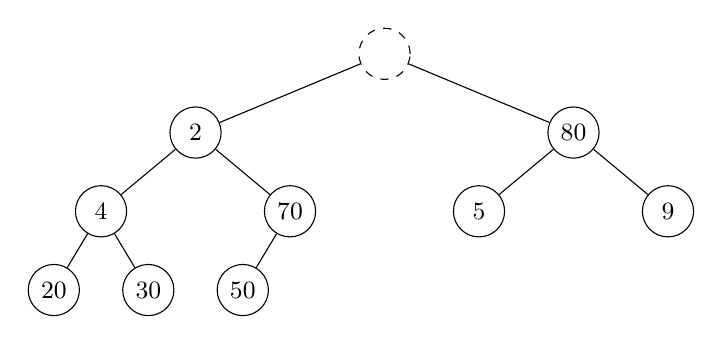
\begin{tikzpicture}[v/.style={circle,draw,minimum size=6.5mm,inner sep=0pt,font=\small},
  level distance=10mm, level 1/.style={sibling distance=48mm}, level 2/.style={sibling distance=24mm},
  level 3/.style={sibling distance=12mm}]
\node[v,dashed] {}
  child {node[v] {2}
    child {node[v] {4} child {node[v] {20}} child {node[v] {30}}}
    child {node[v] {70} child {node[v] {50}} child[missing] {}}}
  child {node[v] {80}
    child {node[v] {5}}
    child {node[v] {9}}};
\end{tikzpicture}
\end{center}
檢查：兄弟對 $(2, 80)$、$(4, 70)$、$(5, 9)$、$(20, 30)$ 都左小右大；$20, 30, 50$ 都夾在祖父（元素 $2$ 所在
節點）的兩個子節點 $4$ 和 $70$ 之間；$4, 70, 5, 9$ 都夾在 $2$ 和 $80$ 之間。

\textbf{㈡ 刪除 $2$}。 $2$ 是最小值，在根的左子節點，就是「刪除最小值」（資結書虛擬碼~8.8 的
\textsc{SMMH-Delete-Min}）。 取出最後一格的 $50$，最後一格變成位置 $9$，洞在位置 $2$：
\begin{enumerate}
\item 洞 $2$：候選是位置 $2$ 和兄弟位置 $3$ 的左子節點，$A[4] = 4$、$A[6] = 5$，較小的是 $4$，$4 < 50$，$4$
上到位置 $2$，洞移到 $4$。 洞的右兄弟 $A[5] = 70$，$50 \le 70$，不用對調。
\item 洞 $4$：候選 $A[8] = 20$（$A[10]$ 已不存在），$20 < 50$，$20$ 上來，洞移到 $8$。 右兄弟 $A[9] = 30 < 50$，
對調：$50$ 放進位置 $9$，手上換成 $30$。
\item 洞 $8$ 沒有子節點，$30$ 放進位置 $8$。
\end{enumerate}
\begin{center}
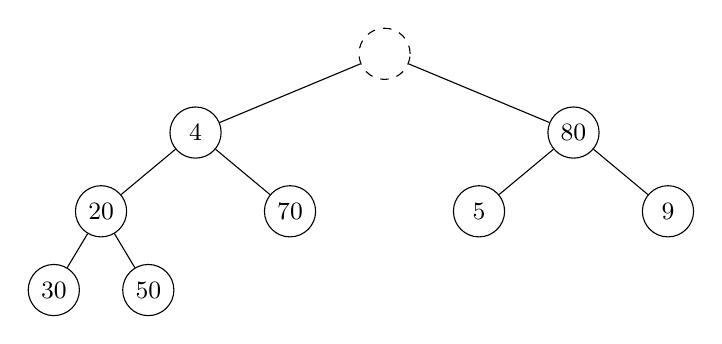
\begin{tikzpicture}[v/.style={circle,draw,minimum size=6.5mm,inner sep=0pt,font=\small},
  level distance=10mm, level 1/.style={sibling distance=48mm}, level 2/.style={sibling distance=24mm},
  level 3/.style={sibling distance=12mm}]
\node[v,dashed] {}
  child {node[v] {4}
    child {node[v] {20} child {node[v] {30}} child {node[v] {50}}}
    child {node[v] {70}}}
  child {node[v] {80}
    child {node[v] {5}}
    child {node[v] {9}}};
\end{tikzpicture}
\end{center}
新的最小值 $4$ 在根的左子節點；$30 \le 50$，兩者都夾在 $4$ 和 $70$ 之間，P1～P3 都成立。

\textbf{㈢ 陣列表示}。 用一維陣列 $A[0..n]$ 依層序存放：根（不放元素）在 $A[0]$，元素放在 $A[1..n]$。 這就是
一般「從 $0$ 起算」的完整二元樹表示法：
\[
\begin{aligned}
p &= \left\lfloor \frac{x - 1}{2} \right\rfloor \quad (x \ge 1), &
g &= \left\lfloor \frac{x - 3}{4} \right\rfloor \quad (x \ge 3), \\
l &= 2x + 1, &
r &= 2x + 2 \quad (\text{索引} \le n \text{ 才存在}), \\
s &= \begin{cases} x + 1, & x \text{ 為奇數（左子節點）}, \\ x - 1, & x \text{ 為偶數（右子節點）}, \end{cases} & &
\end{aligned}
\]
其中 $g = p(p(x))$：$\lfloor(\lfloor(x-1)/2\rfloor - 1)/2\rfloor = \lfloor (x - 3)/4 \rfloor$。 根的子節點
$x = 1, 2$ 沒有祖父；位置 $1$ 起算的版本（資結書）把每個索引加 $1$ 就是了。 在這個陣列裡，P1 寫成「奇數 $x$
有 $A[x] \le A[x + 1]$」，P2、P3 寫成 $A[2g + 1] \le A[x] \le A[2g + 2]$。

㈠ 的 SMMH 存成陣列：
\begin{center}
\small
\begin{tabular}{l*{10}{|c}|}
\cline{2-11}
索引 & 0 & 1 & 2 & 3 & 4 & 5 & 6 & 7 & 8 & 9 \\ \cline{2-11}
$A$ & （空） & 2 & 80 & 4 & 70 & 5 & 9 & 20 & 30 & 50 \\ \cline{2-11}
\end{tabular}
\end{center}
例如 $x = 9$（元素 $50$）：$p = \lfloor 8/2 \rfloor = 4$（元素 $70$），$g = \lfloor 6/4 \rfloor = 1$（元素 $2$），
$s = 10$、$l = 19$ 都超出範圍：$50$ 沒有兄弟也沒有子節點。 又如 $x = 7$（元素 $20$）：$p = 3$（元素
$4$），$g = 1$（元素 $2$），$s = 8$（元素 $30$），$l = 15$ 超出範圍。 檢查 P2、P3：$A[3] = 4 \le 50 \le A[4] = 70$。
\end{pastsoln}
